% !TeX root = ../main.tex
\begin{figure*}[t]
\centering
\begin{subfigure}{\textwidth}
\centering
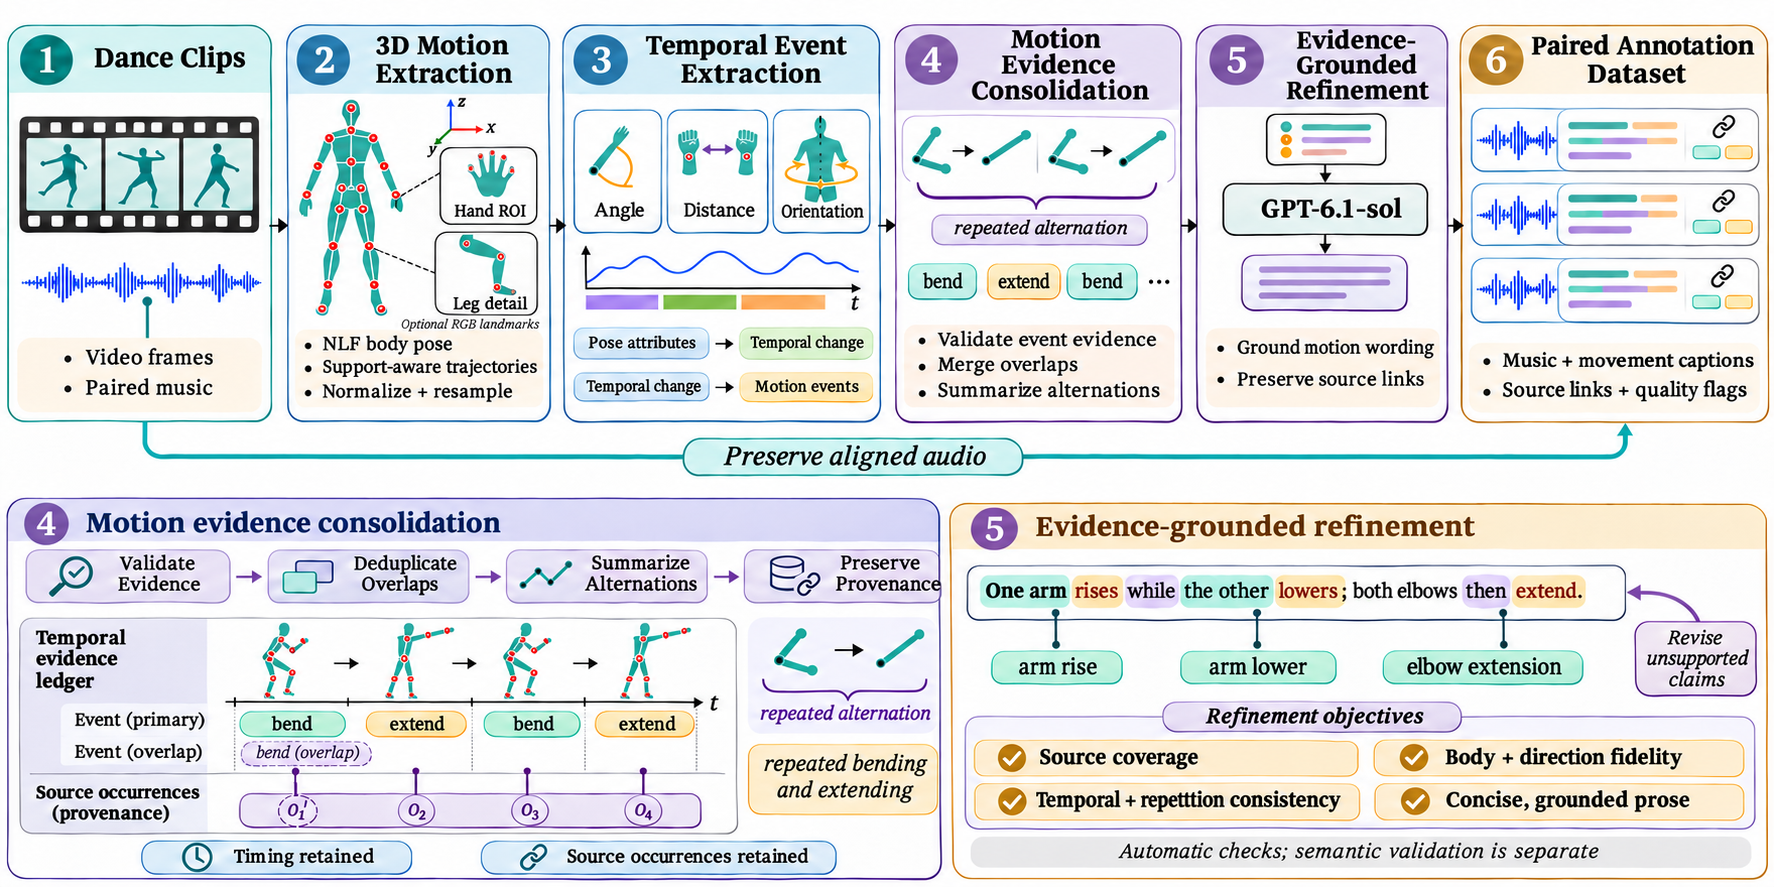
\includegraphics[width=\textwidth]{figures/annotation_pipeline_v5.png}
\caption{Geometry-based annotation framework and evidence-preserving refinement.}
\label{fig:annotation-pipeline}
\end{subfigure}
\par\medskip
\begin{subfigure}{\textwidth}
\centering
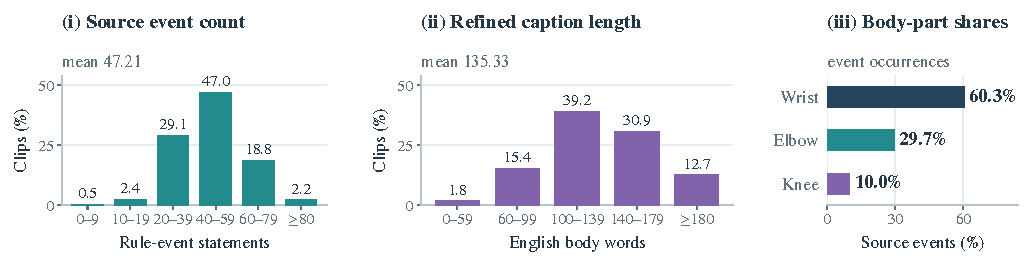
\includegraphics[width=\textwidth]{figures/annotation_distributions_v3.pdf}
\caption{Descriptive statistics on the same 22,352 paired clips.}
\label{fig:annotation-distributions}
\end{subfigure}
\caption{\textbf{Annotation construction and supervision profile.}
(a) MotionScript-based temporal extraction~\cite{motionscript},
Motion Evidence Consolidation, and GPT-6.1-sol evidence-grounded
refinement retain source occurrences and paired music. Hand/leg insets
are detail views; matching 4/5 badges identify expanded stages.
This is a component-integration framework; current experimental labels
come from the existing 2D rule-log rewrite route, detailed in
Appendix~\ref{sec:annotation-details}.
(b) Frozen paired statistics retain all automatic quality flags.
Event occurrences, caption body words, and body-part shares use different
units; they characterize supervision rather than gains in action accuracy
or diversity. The style prefix is excluded from word counts.}
\label{fig:dataset-overview}
\end{figure*}
